\documentclass[pdftex]{beamer} 
% \usepackage[pdftex]{graphicx}
\usepackage{amsmath,amssymb,amsthm} 
%\usepackage[authoryear]{natbib}
%\bibliographystyle{plainnat}
%\setcitestyle{square,aysep={}}
\usepackage{pb-diagram}
\usepackage{ucs}
\usepackage[utf8x]{inputenc}
% \usepackage[russian]{babel}
\usepackage{epstopdf}
\usepackage{multicol}
\usepackage{cancel}

\usepackage{amsfonts}

%%%%%%%%%%%%%%%%%%%%%%%%%%%%%%%%%%%%%%%%%%%%%%%%%%%%%%%%%%%%%%%%%%%%%%%%%%%%%%%%%%%%%%%%%%%%%%%%%%% 

% \newtheorem{theorem}{Theorem}
%% \newtheorem{acknowledgement}[theorem]{Acknowledgement}
%% \newtheorem{algorithm}[theorem]{Algorithm}
%% \newtheorem{axiom}[theorem]{Axiom}
%% \newtheorem{case}[theorem]{Case}
%% \newtheorem{claim}[theorem]{Claim}
%% \newtheorem{conclusion}[theorem]{Conclusion}
%% \newtheorem{condition}[theorem]{Condition}
%% \newtheorem{conjecture}[theorem]{Conjecture}
%% \newtheorem{mycorollary}[theorem]{Corollary}
%% \newtheorem{mycriterion}[theorem]{Criterion}
%% \newtheorem{mydefinition}[theorem]{Definition}
%% \newtheorem{myexample}[theorem]{Example}
%% \newtheorem{myexercise}[theorem]{Exercise}
%% \newtheorem{mylemma}[theorem]{Lemma}
%% \newtheorem{mynotation}[theorem]{Notation}
%% \newtheorem{myproblem}[theorem]{Problem}
%% \newtheorem{myproposition}[theorem]{Proposition}
%% \newtheorem{myremark}[theorem]{Remark}
%% \newtheorem{mysolution}[theorem]{Solution}
%% \newtheorem{mysummary}[theorem]{Summary}
%% \newenvironment{myproof}[1][Proof]{\textbf{#1.} }{\ \rule{0.5em}{0.5em}}


\newcommand{\go}{\stackrel{\circ }{\mathfrak{g}}}
\newcommand{\ao}{\stackrel{\circ }{\mathfrak{a}}}
\newcommand{\co}[1]{\stackrel{\circ }{#1}}
\newcommand{\pia}{\pi_{\mathfrak{a}}}
\newcommand{\piab}{\pi_{\mathfrak{a}_{\bot}}}
\newcommand{\gf}{\mathfrak{g}}
\newcommand{\gfh}{\hat{\mathfrak{g}}}
\newcommand{\af}{\mathfrak{a}}
\newcommand{\afh}{\hat{\mathfrak{a}}}
\newcommand{\bff}{\mathfrak{b}}
\newcommand{\afb}{\mathfrak{a}_{\bot}}
\newcommand{\hf}{\mathfrak{h}}
\newcommand{\hfg}{\hf_{\gf}}
\newcommand{\hfb}{\mathfrak{h}_{\bot}}
\newcommand{\pf}{\mathfrak{p}}
\newcommand{\aft}{\widetilde{\mathfrak{a}}}

% \pagestyle{plain}

\theoremstyle{definition} \newtheorem{Def}{Definition}
\setbeamertemplate{caption}[empty]
\newcommand{\tr}{\hat\triangleright} \newcommand{\trc}{\triangleright}
\newcommand{\adk}{a^{\dagger}_{\kappa}} \newcommand{\ak}{a_{\kappa}}
\def\bF{\mbox{$\overline{\cal F}$}} \def\F{\mbox{$\cal F$}}

\usetheme{default}
% \usetheme{Warsaw}
\title[BCC operators]{Boundary condition changing operators and singular vectors of Virasoro and
affine Lie algebra modules}
\author[Anton Nazarov]{Anton Nazarov}

\institute[SPbSU]{
  Department of high-energy physics,\\
  Faculty of physics,\\ 
  Chebyshev laboratory,\\
  Faculty of mathematics and mechanics,\\
  Saint-Petersburg State University,\\
  198904, Saint-Petersburg, Russia\\
  e-mail: anton.nazarov@hep.phys.spbu.ru
}

\date[Conformal geometry] % (optional, should be abbreviation of conference name)
{Conformal geometry program,\\ Simons center for geometry and physics, April 17, 2013}
\begin{document}
\maketitle

\section{Introduction}
\begin{frame}
  \frametitle{Plan of the talk}
  \begin{itemize}
  \item CFT description of SLE martingales
  \item WZNW models and SLE with random gauge transformations
  \item Martingale condition and singular vectors
  \item Singular vectors and affine Lie algebra module structure
  \item SLE on coset space
  \item Boundary condition changing operators in coset models
  \item Parafermions
  \end{itemize}
\end{frame}
\begin{frame}
  \frametitle{Domain wall in Ising model}
  \vspace{-1cm}  
  \begin{figure}[h]
    \begin{multicols}{2}

      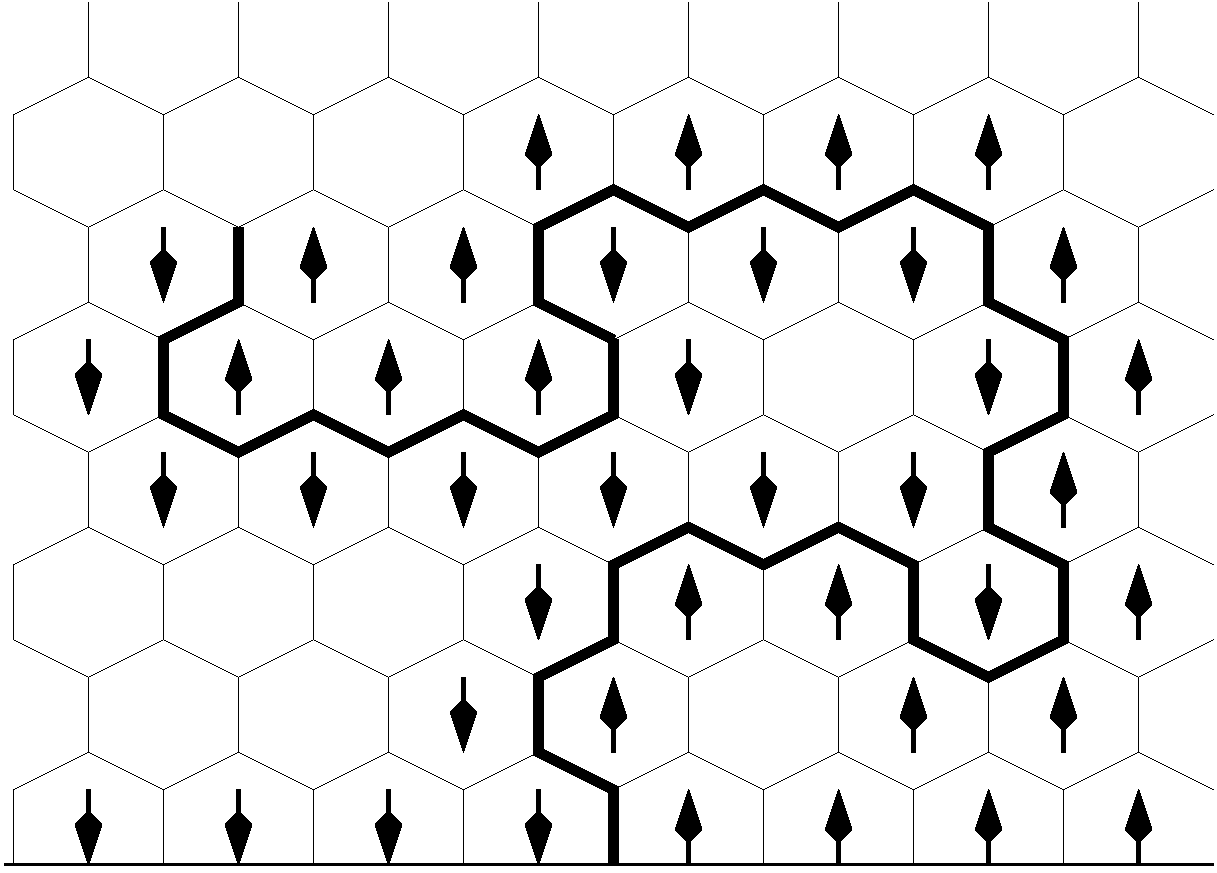
\includegraphics[height=25mm]{explore.pdf}
      \caption{Cut along domain wall}
      \label{fig:sle}

      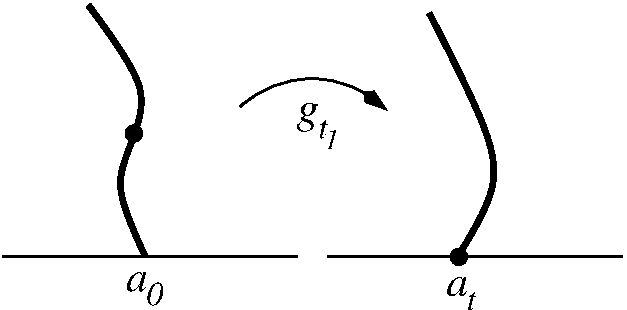
\includegraphics[width=50mm]{loewner.pdf}
      \caption{Conformal map}
      \label{fig:sle}
    \end{multicols}
  \end{figure}    
  \vspace{-1cm}
    {\it Schramm-Loewner evolution} on the upper half-plane $\mathbb{H}$ is a stochastic process which satisfies equation
    \begin{equation*}
      \frac{\partial g_t(z)}{\partial t} = \frac{ 2}{g_t(z)-\sqrt{\kappa}\xi_{t}} \quad \text{or} \quad       d w _{t}= \frac{2dt}{w_{t} }-\sqrt{\kappa}\xi_{t}
    \end{equation*}

  Conformally-invariant probability measure on trajectories $\gamma_{t}$ in $\mathbb{H}$.
  
\end{frame}

\begin{frame}
  \frametitle{CFT description}
  Expectation for a lattice observable $\mathcal{O}$ is averaged over SLE traces:
  \begin{equation*}
    \prec \mathcal{O} \succ_{\mathbb{H}}=\mathbb{E}\left[\prec\mathcal{O}\succ_{\gamma_{t}}\right]=\sum_{\gamma_{t}} P\left[C_{\gamma_{t}}\right] \prec \mathcal{O} \succ_{\gamma_{t}}
  \end{equation*}
  $\prec \mathcal{O} \succ_{\mathbb{H}}$ does not depend on $t$, hence $\prec\mathcal{O}\succ_{\gamma_{t}}$ is a martingale.

  Continuous limit in critical point can be written as CFT correlation function
  \begin{equation*}
    \prec \mathcal{O} \succ_{\mathbb{H}_{t}}\to \mathcal{F}(\left\{z_{i}\right\})_{\mathbb{H}_{t}}=
    \frac{\left< \mathcal{O}(\{z_{i}\})\phi(z_{t})\phi^{\dagger}(\infty)\right>_{\mathbb{H}_{t}}}{\left<\phi(z_{t})\phi^{\dagger}(\infty)\right>_{\mathbb{H}_{t}}}=
    \frac{\left< ^{g_{t}}\mathcal{O}\phi(\xi_{t})\phi^{\dagger}(\infty)\right>_{\mathbb{H}}}{\left<\phi(z_{t})\phi^{\dagger}(\infty)\right>_{\mathbb{H}}}
  \end{equation*}
  Here $\phi$ is boundary condition changing operator. 


   After conformal map $w(z):\mathbb{H}\setminus\gamma_{t}\to \mathbb{H}$
  \begin{equation*}
    \mathcal{F}(\left\{z_{i}\right\})_{\mathbb{H}_{t}}=\prod \left(\frac{\partial w(z_{i})}{\partial z_{i}}\right)^{h_{\lambda_i}} 
    \prod \left(\frac{\partial \bar w(\bar z_{i})}{\partial \bar z_{i}}\right)^{h_{\lambda^{*}_i}}
        \mathcal{F}(\left\{w_{i}, \bar w_{i}\right\})_{\mathbb{H}}
  \end{equation*}
  Consider evolution  $t \to t+dt$. First factor gives $-\frac{2h_{\lambda_{i}}}{w_{i}^{2}}\left(\frac{\partial w_{i}}{\partial z_{i}}\right)^{h_{\lambda_{i}}}$. Fields:
$d\phi_{\lambda_{i}}(w_{i}) = \mathcal{G}_{i}\phi_{\lambda_{i}}(w_{i})=\left(\frac{2dt}{w_{i}}-\sqrt{\kappa} d\xi_{t}\right) \partial_{w_{i}}\phi_{\lambda_{i}}(w_{i})$
\end{frame}
\begin{frame}
  \frametitle{SLE martingales}
  We have
  \begin{equation*}
    \mathbb{E}\left[\prec\mathcal{O}\succ_{\gamma_{t}}\right]=    \mathbb{E}\left[\prec\mathcal{O}\succ_{\gamma_{t+dt}}\right], \quad \mathbb{E}\left[d \prec\mathcal{O}\succ_{\gamma_{t}}\right]=0
  \end{equation*}
  we use Ito formula to get
  \begin{equation*}
\hspace{-0.5cm}    \prod_{i=1}^{2N}\left(\frac{\partial w_{i}}{\partial z_{i}}\right)^{-h_{i}}\mathbb{E}\left[d 
      \mathcal{F}_{\mathbb{H}_{t}}\right]=\left(-\sum_{i=1}^{2N}\frac{2h_{i}dt}{w_{i}^{2}}+\mathbb{E}\left[\sum_{i=1}^{2N}\mathcal{G}_{i}+\frac{1}{2}
        \sum_{i,j}\mathcal{G}_{i}\mathcal{G}_{j}\right]\right)\mathcal{F}_{\mathbb{H}}
  \end{equation*}
  Then use explicit form generators and obtain
  \begin{equation*}
    \left( \sum_{i}\left[-\frac{2h_{i}}{w_{i}^{2}} +\frac{2}{w_{i}}\partial_{w_{i}}\right]+\frac{\kappa}{2}\sum_{i,j}\partial_{w_{i}} \partial_{w_{j}}\right)\mathcal{F}(\left\{w_{i}\right\})=0
  \end{equation*}

  We can rewrite it as the necessary condition on b.c.c. operator $\phi$:
  \begin{equation*}
    (L_{-2}-\frac{\kappa}{2}L_{-1}^{2})\phi=0 \Longrightarrow \phi \left|0\right>  \text{has level 2 null state}, \phi\sim \phi_{1,2} \;\text{or}\; \phi_{2,1}
  \end{equation*}
  Virasoro Verma module $V^{c,h}$ has a level two singular vector.
\end{frame}

%% \begin{frame}
%%   \frametitle{Singular vectors of Virasoro module}
%%   
%% \end{frame}
%% 
\section{SLE and WZNW models}
\label{sec:sle-wzw-models}

\begin{frame}
  \frametitle{WZNW models}
  The action is written in terms of map $g:S^{2}\to \pi(G)$:
  \begin{multline*}
    S=-\frac{k}{8\pi}\int d^2x\; \mathcal{K} (g^{-1}\partial^{\mu}g, g^{-1} \partial_{\mu}g)  
    \\
    - \frac{k }{24\pi^{2}} \int_{B}\epsilon_{ijk} \mathcal{K}\left(
      \tilde g^{-1}\frac{\partial \tilde g}{\partial y^i},\left[
      \tilde g^{-1}\frac{\partial \tilde g}{\partial y^j}
      \tilde g^{-1}\frac{\partial \tilde g}{\partial y^k}\right]\right) d^3y
  \end{multline*}
  \begin{itemize}
  \item   Currents 
    $J(z)= -k \partial_zg g^{-1}\quad \bar J(\bar z)=k g^{-1}\partial_{\bar z}g$

  \item Gauge invariance
    $ g(z,\bar z)\to \Omega(z)g(z,\bar z)\bar \Omega^{-1}(\bar z)$,    where $\Omega,\;\bar \Omega \in G$

  \item Ward identities $\Omega=1+\omega$:
    \begin{equation*}
      \label{eq:87}
      \delta_{\omega,\bar \omega}\left< X \right>=-\frac{1}{2\pi i}\oint dz \sum\omega^a \left< J^a X\right>+
      \frac{1}{2\pi i} \oint d\bar z \sum \bar \omega^a \left< \bar J^a X\right>
    \end{equation*}
  \end{itemize}
\end{frame}

\begin{frame}
  \frametitle{Primary fields}
  \begin{itemize}
  \item Mode expansion gives commutation relations of affine Lie algebra $\gfh$: 
    \begin{equation*}
      \left[J^a_n,J^b_m\right]=\sum_c i f^{abc}J^c_{n+m}+kn\delta^{ab}\delta_{n+m,0} \; \text{where} \;           J^a(z)=\sum\limits_{n\in \mathbb Z}z^{n-1}J^a_n 
    \end{equation*}
  \item Sugawara construction $  L_n=\frac{1}{2(k+h^{\vee}_{\gf})}\sum\limits_a\sum\limits_m:J^a_m J^a_{n-m}:$ -- embedding $Vir\subset U(\gfh)$.
  \item Chiral algebra $\gfh \ltimes Vir$:
    \begin{equation*}
      \label{eq:92}
      \begin{aligned}
        \left[L_n,L_m\right]=(n-m)L_{n+m}+\frac{k\mathrm{dim}\gf}{(k+h^{\vee}_{\gf})}\frac{(n^3-n)}{12}\delta_{n+m,0}\\
        \left[L_n,J^a_m\right]=-mJ^a_{n+m}
      \end{aligned}
    \end{equation*}

  \item Primary fields $\phi_{\lambda}$ are labeled by highest weights of representations
    ($\{t^{a}_{\lambda}\}$ --orthonormal basis):
    \begin{equation*}
      \begin{aligned}
        & J_0^a\left|\phi_{\lambda}\right>=-t^a_{\lambda}\left|\phi_{\lambda}\right>  \quad    J^a_n\left|\phi_{\lambda}\right>=0 \quad \mbox{for}\; n>0 \\
        & L_0\left|\phi_{\lambda}\right>=\frac{1}{2(k+h^{\vee}_{\gf})}\sum_aJ^a_0J^a_0\left|\phi_{\lambda}\right>=\frac{(\lambda,\lambda+2\rho)}{2(k+h^{\vee}_{\gf})}\left|\phi_{\lambda}\right>=h_{\lambda} \left|\phi_{\lambda}\right>
      \end{aligned}
    \end{equation*}
  \end{itemize}
\end{frame}

\begin{frame}
  \frametitle{SLE and WZNW models}
  Similarly to minimal models we consider an observable
  \begin{equation*}
    \mathcal{F}(\left\{z_{i}\right\})_{\mathbb{H}_{t}}=
    \frac{\left<\phi_{\Lambda}(z_{t}) \phi_{\lambda_1}(z_{1}) \dots \phi_{\lambda_n}(z_{n}) \phi_{\lambda^{*}_1}(\bar z_{1}) \dots \phi_{\lambda^{*}_n}(\bar z_{n})
        \phi_{\Lambda^{*}}(\infty)\right>}{\left<\phi_{\Lambda}(z_{t})\phi_{\Lambda^{*}}(\infty)\right>}
  \end{equation*}
  Use a conformal map $w(z):\mathbb{H}\setminus\gamma_{t}\to \mathbb{H}$
  \begin{equation*}
    \mathcal{F}(\left\{z_{i}\right\})_{\mathbb{H}_{t}}=\prod \left(\frac{\partial w(z_{i})}{\partial z_{i}}\right)^{h_{\lambda_i}} 
    \prod \left(\frac{\partial \bar w(\bar z_{i})}{\partial \bar z_{i}}\right)^{h_{\lambda^{*}_i}}
        \mathcal{F}(\left\{w_{i}, \bar w_{i}\right\})_{\mathbb{H}}
  \end{equation*}
  Consider evolution from $t$ to $t+dt$. First factor: $-\frac{2h_{\lambda_{i}}}{w_{i}^{2}}\left(\frac{\partial w_{i}}{\partial z_{i}}\right)^{h_{\lambda_{i}}}$. For fields we have
  \begin{equation*}
    d\phi_{\lambda_{i}}(w_{i}) = \mathcal{G}_{i}\phi_{\lambda_{i}}(w_{i})
  \end{equation*}
  But now we need to add random motion in $G$ to stochastic evolution \cite{bettelheim2005stochastic}:
  \begin{equation*}
    \mathcal{G}_{i}=\left(\frac{2dt}{w_{i}}-\sqrt{\kappa}
      d\xi_{t}\right) \partial_{w_{i}}+\frac{\sqrt{\tau}}{w_{i}}\sum_{a=1}^{\mathrm{dim} \gf}\left(d
      \theta ^{a} t^{a}_{i}\right)\quad \mathbb{E}[d\theta^{a} d\theta^{b}]=\delta^{ab} dt
  \end{equation*}
\end{frame}
\begin{frame}
  \frametitle{SLE martingales in WZNW models}
   For martingales we have
  \begin{equation*}
    \left(-2 \mathcal{L}_{-2}+\frac{1}{2}\kappa \mathcal{L}_{-1}^{2}+\frac{1}{2}\tau\sum_{a} \mathcal{J}^{a}_{-1} \mathcal{J}^{a}_{-1}\right)        \mathcal{F}(\left\{w_{i}, \bar w_{i}\right\})_{\mathbb{H}}=0
  \end{equation*}
  \begin{equation*}
    \mathcal{L}_{-n}=\sum_{i}\left(\frac{(n-1)h_{\lambda_{i}}}{(w_{i}-z)^{n}}-\frac{1}{(w_{i}-z)^{n-1}}\partial_{w_{i}}\right);\quad \mathcal{J}^{a}_{{-n}}=-\sum_{i}\frac{t^{a}_{i}}{(w_{i}-z)^{n}}
  \end{equation*}
  so 
  \begin{equation*}
\left| \psi\right>=\left(-2 L_{-2}+\frac{1}{2}\kappa L_{-1}^{2}+\frac{1}{2}\tau\sum_{a} J^{a}_{-1} J^{a}_{-1}\right) \left|\phi_{\Lambda}\right>    
  \end{equation*}
 is level two null state and $J^{a}_{1} \left|\psi\right>=0, J^{a}_{2}\left|\psi\right>=0$. Then $\kappa+\tau h^{\vee}=4$ and it is possible to derive additional relations connecting $\kappa, \tau, k$:
 \begin{equation*}
   \kappa=\frac{2(h^{\vee}-2k)}{2h_{\Lambda}h^{\vee}-k},\quad \tau=\frac{8 h_{\Lambda}-2}{2h_{\Lambda}h^{\vee}-k}  \quad\text{for}\; k\neq 2h_{\Lambda}h^{\vee}
 \end{equation*}
 To get complete classification use Knizhnik-Zamolodchikov equations \cite{alekseev2010sle}.
\end{frame}
%% \begin{frame}
%%   \frametitle{Null states and singular vectors of affine Lie algebra module}
%% 
%%   If $\phi_{\Lambda}$ is primary and $\Lambda$ -- highest weight of integrable representation,
%%   singular vectors are 
%% 
%%   Weyl-Kac character formula for irreducible $\gfh$-module $L^{\mu}$: $\mathrm{ch} L^{\mu}=\frac{\sum_{\omega\in W_{\gfh}} \epsilon(\omega)
%%     e^{\omega(\mu+\rho)-\rho}}{\prod_{\alpha\in \Delta^{+}_{\gfh}}
%%     (1-e^{-\alpha})^{\mathrm{mult}(\alpha)}}$
%% 
%%   $J^{\alpha}\left|\omega(\mu+\rho)-\rho\right> = 0\quad \forall \alpha\in \Delta^{+}_{\gfh}$
%%   %
%%   % Here I need to tell that each null state corresponds to singular vector.
%%   % Then I present Weyl-Kac character formula and describe singular element using Weyl group
%%   % After that I can analyze some example, e.g. sl(n)
%%   % 
%%    %%     Мы продемонстрируем другой подход к анализу соотношения (\ref{eq:16}). С точки зрения
%%    %%     конечномерной подалгебры $\gf\subset\gfh$ все три слагаемых, действующих на состояние
%%    %%     $\left|\phi_{\Lambda}\right>$ в формуле (\ref{eq:16}), являются квадратичными операторами Казимира
%%    %%     (пропорциональны $\sum_a J^a J^a$). Поэтому состояние $\left|\psi\right>$ отвечает весу
%%    %%     $\Lambda-2\delta$.
%%    %%   
%%    %%     Из этого следует необходимое условие на уровень и старший вес $\Lambda$: вектор веса
%%    %%     $\Lambda-2\delta$ должен содержаться в модуле Верма $V^{\mu}_{\gfh}$, старший вес которого
%%    %%     $\mu=w(\Lambda+\rho)-\rho$ является сингулярным для неприводимого модуля $L^{\Lambda}_{\gfh}$. То
%%    %%     есть должны существовать неотрицательные числа $a_0,\dots,a_r\in \mathbb{Z}_+$
%%    %%     ($r=\mathrm{rank}(\gf)$) такие, что
%%    %%   \begin{equation}
%%    %%     \Lambda-2\delta = \mu-\sum_{k=0}^r a_k \alpha_k.
%%    %%   \label{eq:109}
%%    %%   \end{equation} 
%%    %%   Рассмотрим сингулярные веса с минимальным грейдом, которые могут входить в правую часть уравнения
%%    %%   (\ref{eq:109}). Во-первых, это сингулярные веса в нулевом грейде, которые совпадают с сингулярными
%%    %%   весами неприводимого модуля $L^{\Lambda}$ конечномерной алгебры $\gf$. Так как $\alpha_0 =
%%    %%   \delta-\theta$ получаем в этом случае, что $a_0=2$ и $\Lambda-\mu= 2\theta-\sum_{k=1}^r a_k
%%    %%   \alpha_k, \; a_k\geq 0$. В случае алгебры $\gf=\mathfrak{su}(2)$ имеем $\Lambda=l\omega_1,\;
%%    %%   \theta=2\omega_1,\; \rho=\omega_1,\; \mu=-(l+2)\omega_1$ и $2l+2=4-2a_1$. То есть $a_1=0$ и $l=1$, а
%%    %%   поле $\phi_{\Lambda}$ имеет спин $\frac{1}{2}$. В случае алгебры $\gf=\mathfrak{su}(N)$ аналогичное
%%    %%   рассуждение выполняется для каждого из индексов Дынкина, отличных от нуля. То есть равенство
%%    %%   (\ref{eq:109}) может выполняться только если каждый из индексов Дынкина не более единицы.
%%    %%   
%%    %%   Вспомним, что группа Вейля аффинной алгебры Ли $\gfh$ представляет собой полупрямое произведение
%%    %%   группы Вейля конечномерной алгебры $\gf$ и группы трансляций $T=\left\{t_{\alpha_k}\right\}$,
%%    %%   порожденной простыми корнями $\alpha_1,\dots,\alpha_r$. Так как
%%    %%   $t_{\alpha}\lambda=\lambda+\frac{2(\lambda,\delta)}{(\alpha,\alpha)}\alpha-\left(\frac{(\alpha,\alpha)}{2}
%%    %%     (\lambda,\delta)+(\lambda,\alpha)\right) \delta$, в случае длинного корня $\alpha:\;
%%    %%   (\alpha,\alpha)=2$ при $k>2$ и $(\alpha,\lambda)\neq 0$ условие (\ref{eq:109}) не может выполняться
%%    %%   для $\mu=t_{\alpha} w(\Lambda+\rho)-\rho, \; w\in W_{\gf}$ просто в силу того, что грейд в правой
%%    %%   части меньше $-2$.
%%    %%   
%%    %%   Таким образом условие (\ref{eq:109}), характеризующее структуру сингулярного элемента представления
%%    %%   аффинной алгебры Ли $\gfh$, исключает из рассмотрение большое количество примарных полей
%%    %%   $\phi_{\Lambda}$. Вместе с тем это условие несколько слабее, чем необходимые условия, полученные в
%%    %%   разделе 2 работы \cite{alekseev2010sle}.
%% 
%%   
%% \end{frame}
\section{Coset models}
\label{sec:coset-models}

\begin{frame}
  \frametitle{Gauged WZNW-models and coset construction}
  Add gauge fields $A, \bar{A}$ taking values in Lie algebra $\af\subset \gf$ to the action:
  \begin{multline*}
    S(g,A)=S_{WZNW}(g)+\\
    \frac{k}{4\pi}\int d^{2}z \left(\mathcal{K}(A, g^{-1}\bar \partial g)-\mathcal{K}(\bar A, (\partial g ) g^{-1})+\mathcal{K}(A,g^{-1}\bar A g)-\mathcal{K}(A,\bar A)\right)
  \end{multline*}

  Currents:  $J_{(\gf,\af)}=-k\partial g g^{-1} -k g A g^{-1}$

  Ward identities:
  $   \left< A^{b}(z)\phi_{1}\dots \phi_{N}\right>=\frac{2}{k+2
    h^{\vee}_{\af}}\sum_{k}\frac{\tilde{t}^{b}_{k}}{z-z_{k}}\left<\phi_{1}\dots \phi_{N}\right>$ 
  Remember that in WZNW we had OPE: $J_{\gf}^{a}(z)\phi_{i}(w)\sim \frac{-t^{a}_{i}\phi(w)}{z-w}$.
%%  Commutation relations for current components are preserved.

  Algebraic structure is connected with two affine Lie algebras $\gfh, \afh: \afh\subset\gfh$. 

 Virasoro generators are given by difference of Sugawara expressions:
  \begin{equation*}
    L_{n}=L_{n}^{\gf}-L_{n}^{\af}=\frac{1}{2(k+h^{\vee}_{\gf})}\sum\limits_{a,m}:J^a_m J^a_{n-m}: - \frac{1}{2(k+h^{\vee}_{\af})}\sum\limits_{b,m}:\tilde{J}^b_m \tilde{J}^b_{n-m}:
  \end{equation*}

\end{frame}

\begin{frame}
  \frametitle{Primary fields}

  Primary fields are labeled by pairs of weights $(\mu,\nu)\in \hf_{\gfh}\oplus \hf_{\afh}$, such that branching functions $b^{\mu}_{\nu}(q)\neq 0$. But some pairs are equivalent. This equivalence is given by the action of simple currents $(J,\tilde{J})$ such that $h_{J}-h_{\tilde{J}}=0$. 

  Conformal weight of primary field
  \begin{multline}
    L_0\left|\phi_{(\mu,\nu)}\right>=\left(\frac{1}{2(k+h^{\vee}_{\gf})}\sum_aJ^a_0J^a_0-\frac{1}{2(k+h_{\af}^{\vee})}\sum_b \tilde{J}^b_0 \tilde{J}^b_0 \right)
    \left|\phi_{\lambda}\right>=\\
    \left(\frac{(\mu,\mu+2\rho)}{2(k+h^{\vee}_{\gf})}-\frac{(\nu,\nu+2\rho_{\af})}{2(k+h^{\vee}_{\af})}\right)\left|\phi_{(\mu,\nu)}\right>
  \end{multline}

%%  So $G/A$-coset theory is related to $\gf\oplus \bar{\af}$-theory.

 It is possible to obtain analogues of KZ-equations:
  \begin{equation*}
    \left\{\frac{1}{2}\partial_{i} + \sum_{i\neq j}^{N}\left(\frac{t^{a}_{i}t^{a}_{j}}{k+h^{\vee}_{\gf}}-\frac{\tilde t^{b}_{i}\tilde t^{b}_{j}}{k+h^{\vee}_{\af}}\right)\frac{1}{z_{i}-z_{j}}\right\} \left<\phi_{1}(z_{1})\dots \phi_{N}(z_{N})\right>=0
  \end{equation*}
\end{frame}

\begin{frame}
\vspace{-1cm}
  \frametitle{SLE on coset space}
  \begin{multline*}
    \hspace{-1.3cm}
    \prod_{i=1}^{2N}\left(\frac{\partial w_{i}}{\partial z_{i}}\right)^{-h_{i}}\mathbb{E}\left[d 
      \mathcal{F}_{\mathbb{H}_{t}}\right]=
    \left(-\sum_{i=1}^{2N}\frac{2h_{i}dt}{w_{i}^{2}}+\mathbb{E}\left[\sum_{i=1}^{2N}\mathcal{G}_{i}+\frac{1}{2}
        \sum_{i,j}\mathcal{G}_{i}\mathcal{G}_{j}\right]\right)\mathcal{F}_{\mathbb{H}} = 0
  \end{multline*}
  Fix gauge. The generator of field transformation is:
$\mathcal{G}_{i}=\left(\frac{2dt}{w_{i}}-\sqrt{\kappa}
  d\xi_{t}\right) \partial_{w_{i}}+\frac{\sqrt{\tau}}{w_{i}}\left(\sum\limits_{a:\mathcal{K}(t^{a},\tilde{t}^{b})=0}\left(d
    \theta ^{a} t^{a}_{i}\right)\right)$, where  $\mathbb{E}[d\theta^{a}d\theta^{b}]=\frac{dt}{\mathcal{K}(t^{a},t^{b})}$
%%    Подставляем явный вид конформного преобразования полей и получаем равенство
%%    \begin{equation*}
%%      \left( \sum_{i}\left[-\frac{2h_{i}}{w_{i}^{2}} +\frac{2}{w_{i}}\partial_{w_{i}}\right]+\frac{\kappa}{2}\sum_{i,j}\partial_{w_{i}} \partial_{w_{j}}\right)\mathcal{F}(\left\{z_{i}\right\})=0
%%    \end{equation*}
%%  
%%    Можно переписать в виде соотношений на оператор смены граничных условий $\phi$:
%%    \begin{equation*}
%%      (L_{-2}-\frac{\kappa}{2}L_{-1}^{2})\phi=0 \Longrightarrow \phi \left|0\right>  \text{has level 2 null state}, \phi\sim \phi_{1,2} \;\text{or}\; \phi_{2,1}
%%    \end{equation*}
%%  

%%   For  $\gf\oplus \af$ WZNW-model we can write SLE generator of primary field transformation under stochastic evolution as
%%   \begin{equation*}
%%     \mathcal{G}_{i}=\left(\frac{2dt}{w_{i}}-\sqrt{\kappa} d\xi_{t}\right) \partial_{w_{i}}+\frac{\sqrt{\tau}}{w_{i}}\left(\sum_{a=1}^{\mathrm{dim} \gf}\left(d \theta ^{a} t^{a}_{i}\right)+\sum_{b=1}^{\mathrm{dim} \af}\left(d \tilde{\theta} ^{b} \tilde{t}^{b}_{i}\right)\right)
%%   \end{equation*}
%%    \begin{equation*}
%%      \mathcal{G}_{i}^{L,R}=\left(\frac{2dt}{w_{i}}-\sqrt{\kappa} d\xi_{t}\right) \partial_{w_{i}}+\frac{\sqrt{\tau}}{w_{i}}\left(\sum_{a=1}^{\mathrm{dim} \gf}\left(d \theta ^{a} t^{a}_{i}\right)\pm\sum_{b=1}^{\mathrm{dim} \af}\left(d \tilde{\theta} ^{b} \tilde{t}^{b}_{i}\right)\right)
%%    \end{equation*}

Substitute to martingale condition
  \begin{equation*}
    \left(-2 \mathcal{L}_{-2}+\frac{1}{2}\kappa \mathcal{L}_{-1}^{2}+\frac{\tau}{2}\left( \sum_{a} \mathcal{J}^{a}_{-1} \mathcal{J}^{a}_{-1}-
        \sum_{b}\tilde{\mathcal{J}}^{b}_{-1} \tilde{\mathcal{J}}^{b}_{-1}\right)\right)        \mathcal{F}_{\mathbb{H}}=0
  \end{equation*}

which can be rewritten as the requirement for
\begin{equation*}
  \psi=\left(-2L_{-2}+\frac{1}{2}\kappa L_{-1}^{2}+\frac{1}{2}\tau \left(\sum_{a=1}^{\mathrm{dim}\gf}J^{a}_{-1}J^{a}_{-1}-\sum_{b=1}^{\mathrm{dim}\af}\tilde{J}^{b}_{-1}\tilde{J}^{b}_{-1}\right)\right) \phi_{(\mu,\nu)}
\end{equation*}
to be level two null-field.
\end{frame}

\begin{frame}
  \frametitle{Solutions of martingale condition}
  Applying $L_{2}^{\gf}$ we get
  \begin{equation*}
    L_{2}^{\gf}\psi= \left(-8 L_{0}-c+ 3 \kappa L_{0}+\frac{1}{2}\tau (k \dim\gf-x_{e}k\dim\af)\right) \varphi_{(\mu,\nu)}=0
  \end{equation*}
  We use $L_{0} \varphi_{(\mu,\nu)}=h_{(\mu,\nu)} \varphi_{(\mu,\nu)}$, with the conformal weight  $h_{(\mu,\nu)}= \left(\frac{(\mu,\mu+2\rho)}{2(k+h^{\vee}_{\gf})}-\frac{(\nu,\nu+2\rho_{\af})}{2(k x_{e}+h^{\vee}_{\af})}\right)$ and the central charge $c=\frac{k\dim \gf}{k+h^{\vee}_{\gf}}-\frac{x_{e}k\dim \af}{x_{e} k+h^{\vee}_{\af}}$. This leads to the relation on $\kappa,\tau$:
  \begin{equation*}
    \label{eq:28} (3\kappa-8)h_{(\mu,\nu)}-c+\tau (k\dim\gf-x_{e}k\dim\af) =0.
  \end{equation*}
  The second relation appears as a result of the $L_{1}^{\gf}$-action:
  \begin{equation*}
    \label{eq:21}
    -12 h_{(\mu,\nu)}+2\kappa h_{(\mu,\nu)} (2h_{(\mu,\nu)}+1) + \tau
    (C_{\mu}-\tilde{C}_{\nu})=0,
  \end{equation*}
  where $C_{\mu}=(\mu,\mu+2\rho)$ and $\tilde{C}_{\nu}=(\nu,\nu+2\rho_{\af})$ are the eigenvalues of the quadratic Casimir operators $\sum_{a}t^{a}t^{a}$ and $\sum_{b}\tilde{t}^{b}\tilde{t}^{b}$ of Lie algebras $\gf$ and $\af$.
  So we obtain the necessary conditions for CFT correlation functions to be SLE martingales. 

  We immediately get $\kappa,\tau$ for each pair $(\mu,\nu)$ of $\gf$ and $\af$-weights. 

\end{frame}

\begin{frame}
  \frametitle{Parafermions}
  $\mathbb{Z}(N)$ parafermions are equivalent to $SU(2)_{N}/U(1)$ coset theory.
  
  Parafermionic field decomposes as
  \begin{equation*}
    \Phi^{j}=\phi_{j}(z) \exp\left( -i \frac{j}{\sqrt{N}}\phi(z)\right)
  \end{equation*}
  where $\phi_{j}(z)$ is field of $SU(2)$-WZNW model with spin $j$, $\phi(z)$ -- $U(1)$ bosonic field.
  
  For parafermionic current we have
  \begin{equation*}
    \Psi^{\pm}=\frac{1}{\sqrt{N}} J^{\pm}\exp\left(\mp i \frac{1}{\sqrt{N}}\phi(z)\right)
  \end{equation*}
%%  Its action in terms of primary fields of $su(2)\oplus u(1)$ WZNW-model is equivalent to $J^{\pm}\pm \tilde{J}^{\pm}$.

  Martingale condition can be rewritten as
  \begin{equation*}
    \left(-2 L_{-2}+\frac{\kappa}{2}L_{-1}^{2}+\frac{\tau}{2}\left[\Psi^{+}_{-1}\Psi^{-}_{-1}+\Psi^{-}_{-1}\Psi^{+}_{-1}\right]\right) \left|\Phi\right>=0
  \end{equation*}
  which coincides with the result of Santachiara [arXiv:0705.2749].
\end{frame}
\begin{frame}
  \frametitle{Solutions for parafermions and minimal models}
  The central charge is $c=\frac{3N}{N+2}-1=\frac{2N-2}{N+2}$. Conformal weights of primary fields with Dynkin indeces $(k,l)$ are $h_{(k,l)}=\frac{k(k+2)}{4(N+2)}-\frac{l^{2}}{4N}$.

  \begin{itemize}
  \item $N=2$, $c=\frac{1}{2}$ corresponds to the Ising model. Non-trivial primary fields with
    weights $h_{(2,0)}=1/2, h_{(1,1)}=1/16$.   
    Substituting the field $\varphi_{(2,0)}$  we get: $3\kappa-9+4\tau =0;\quad -3+\kappa+4\tau=0$.
    The solution is $\kappa=3, \tau=0$. For the field $\varphi_{(1,1)}$ the relations are
    $3\kappa-16+64\tau=0,\quad -64+9\kappa + 64\tau=0$, $\kappa=16/3, \tau=0$. 

    No additional motion for the Ising model.
  \item $N=3$ parafermionic model, central charge is $c=\frac{4}{5}$. Conformal weights are
    $h_{(0,0)}=0$, $h_{(0,2)}=h_{(0,-2)}=\frac{2}{3}\; \mathrm{mod}\; 1$, $h_{(2,0)}=\frac{2}{5}$,
    $h_{(2,2)}=h_{(2,-2)}=\frac{1}{15}$.  Solutions $(\kappa,\tau)$:
    $(\frac{208}{25},\frac{242}{225}), (\frac{10}{3},0),(\frac{80}{19},\frac{14}{171})$. 

    Field $\varphi_{(2,0)}$ constitutes the $Z_{3}$-singlet, so  an additional random walk does not
    appear and $\tau=0$.

  \item 
    For $\frac{\hat{su}(2)_{N}\oplus \hat{su}(2)_{1}}{\hat{su}(2)_{N+1}}$-coset realization of minimal unitary models the system of equations is always consistent for $\tau=0$.
  \end{itemize}

\end{frame}
%% \begin{frame}
%% 
%%   \frametitle{Next steps}
%%   \begin{itemize}
%%   \item Act on $  \psi=\left(-2L_{-2}+\frac{1}{2}\kappa L_{-1}^{2}+\frac{1}{2}\tau \left(\sum\limits_{a=1}^{\mathrm{dim}\gf}J^{a}_{-1}J^{a}_{-1}+\sum\limits_{b=1}^{\mathrm{dim}\af}\tilde{J}^{b}_{-1}\tilde{J}^{b}_{-1}\right)\right) \phi_{(\Lambda,\Gamma)}$ with $J^{(a,b)}_{1}, J^{(a,b)}_{2}$ and get relations connecting $\kappa, \tau, k$. 
%%   \item Use Knizhnik-Zamolodchikov equations to simplify them.
%%   \item Get conditions on boundary condition changing operator
%%   \item Compare these conditions with results of  the study of boundary states with fusion algebra (Verlinde formula for Cardy states)
%%   \end{itemize}
%% \end{frame}
%% 
\section{Conclusion}
\label{sec:conclusion}


\begin{frame}
  \frametitle{Conclusion and outlook}
  \begin{itemize}
  \item Martingale conditions are equivalent to Verma module of Virasoro or affine Lie algebra having singular weights at level two.
  \item Coset conformal field theory correlation functions satisfy martingale conditions for
    Schramm-Loewner evolution with random walk on coset space $G/A$.
  \item Perturbation of coset model: $
    S_{\text{pert}}=S_{G/A}(\gamma,\alpha)-\frac{k\lambda}{2\pi}\int {\cal K} (\gamma T, \gamma^{-1}
    \bar T),\quad  T,\bar T\in \gf - \mathrm{fixed}$. It is an affine Toda field theory. Can it be
    connected with massive SLE?
  \item Full solution, comparison with b.c.c. classification from Cardy conditions.
  \end{itemize}
\end{frame}

\begin{frame}[c,plain]
  \begin{center}
  \Large{Thank you for your attention!}
  \end{center}
\end{frame}

\bibliography{bibliography}{} 
\bibliographystyle{apalike}
\end{document}
